% ==============================================================================
% LAB 119
% UNDERSÖKNING AV RC-KRETS
% ------------------------
%
% Author:
% Jonas Sjöberg     <tel12jsg@student.hig.se>
%
% License:
% Creative Commons Attribution-NonCommercial-ShareAlike 4.0 International
% See LICENSE.md for full licensing information.
% ==============================================================================

\section{Introduktion}\label{intro}
% ------------------------------------------------------------------------------
I denna labb skall vi studera en passiv krets uppbyggd av ett motstånd och en
kondensator. Om en sådan krets matas med en sinusformad insignal kommer den att
släppa igenom vissa frekvenser medan andra frekvenser dämpas. Ett sådant
frekvensberoende nät kallas därför ofta för filter. Om kretsen innehåller
endast en reaktiv (dvs energilagrande) komponent (spole eller kondensator)
kallar vi kretsen för ett första ordningens filter. Namnet kommer sig av att
kretsen kan beskrivas med en första ordningens differentialekvation.  Vi skall
analysera kretsen både i frekvensplanet genom att mäta upp ett Bode-diagram och
i tidsplanet genom att mäta upp kretsens stegsvar.  Ett första ordningens
lågpassfilter kan konstrueras enligt Figur~\ref{fig:rc-schema}.

\section{Lågpassfilter}
\subsection{Överföringsfunktion}
% ------------------------------------------------------------------------------
Uttryck~\eqref{eq:transfer} beskriver lågpassfiltrets överföringsfunktion i
Bodes normalform.

\begin{equation*}
  \begin{split}
    H(j\omega) &= \dfrac{U_{ut}}{U_{in}}                                      \\
               &= \dfrac{\dfrac{1}{\jmath\omega C}}{R + \dfrac{1}{j\omega C}} \\
               &= \dfrac{1}{1+\jmath\omega R C}                               \\
  \end{split}
\end{equation*}

\begin{equation}\label{eq:transfer}
  H(j\omega) = \dfrac{1}{1+j(\omega/\omega_1)}
\end{equation}

där $\omega_1 = \tfrac{1}{R C}$ är brytfrekvensen uttryckt som en
vinkelfrekvens $\si{\radian\per\second}$.


\par
Eftersom $\omega = 2 \pi f$ kan vi också uttrycka överföringsfunktionen som:

\begin{equation*}
  \begin{split}
    H(f) &= \dfrac{U_{ut}}{U_{in}}        \\
    H(f) &= \dfrac{1}{1+\jmath 2 \pi R C} \\
  \end{split}
\end{equation*}

\begin{equation}\label{eq:transfer2}
  H(f) = \dfrac{1}{1+\jmath (\dfrac{f}{f_1})}\
  \text{där}\ f_1 = \dfrac{1}{2 \pi R C} \si{\Hz}
\end{equation}


\par Den senare formen, ekv.~\eqref{eq:transfer2} är att föredra när man
plottar upp överföringsfunktionen från mätresultatet och är den form vi
använder i labben.

Eftersom överföringsfunktionen är på komplex form har den både absolutbelopp
och fasvinkel, ekv.~\eqref{eq:complexform}:

\begin{equation}\label{eq:complexform}
  \begin{split}
    |H(f)| &= \dfrac{1}{\sqrt{1+{(\frac{f}{f_1})}^2}} \\
      ArgH &= -\arctan{\frac{f}{f_1}}
  \end{split}
\end{equation}

%$z = 1.19 \phase{-78.2039^{\circ}}$


\section{Experimentuppställning}\label{}
% ------------------------------------------------------------------------------
En så kallad experimentplatta eller ``breadboard'' används för att konstruera
kretsen som illustreras i Figur~\ref{fig:rc-schema}.  \par För att generera en
sinusformad signal används signalgeneratorn \texttt{HP33120A}, vars utgång
kopplas genom en BNC-förgrening till oscilloskopet \texttt{Agilent 54621A} och
genom en BNC- banankontaktadapter, med ``banankablar'' till breadboardplattans
skruvterminaler.  \par Oscilloskopets första kanal visar signalen från kretsens
ingång, punkten \texttt{Vout} i Figur~\ref{fig:rc-schema}. Samma punkt utgör
signalgeneratorns utgång och vid några mätningar användes en T-koppling av
BNC-kablar för att mata signalgeneratorns utgång till både experimentkopplingen
och oscilloskopet.  En oscilloskopprob är ansluten till oscilloskopets andra
kanal. Proben kopplas till kretsens utgång, punkten \texttt{Vout} i
Figur~\ref{fig:rc-schema} med en oscilloskop-prob. Proben ställs till att dämpa
med en faktor av 10:1 och den vertikala skalan justeras en dekad nedåt, så att
båda kanalerna visas med samma skalfaktor.
\par Impedansskillnaden mellan signalgenerator, kablage och mätutrustning antas
vara hög nog för att inte ha någon avgörande inverkan på mätresultaten. Detta
återkommer i Sektion~\ref{impedans}.

\begin{figure}\label{fig:rc-schema}
  \centering
  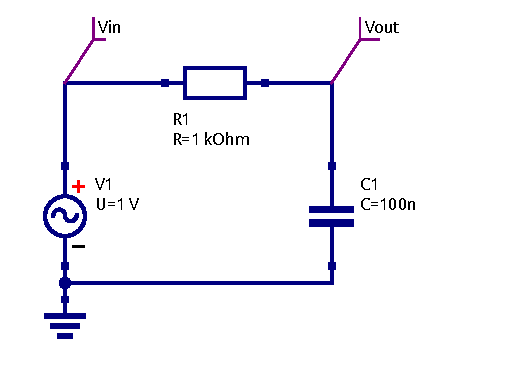
\includegraphics[width=0.8\linewidth]{sim/ee466_lab-4_prj/uppgift-0_schema}
  \caption[Schematisk ritning av labbkoppling, första ordningens RC-filter.]
  {Schematisk ritning av labbkoppling, första ordningens RC-filter.}
\end{figure}

De värden som presenteras i rapporten uppmättes med ett analogt 2-kanals
oscilloskop \texttt{Hitachi V-252} med en bandbredd på \SI{20}{\MHz}.  Signalen
genererades av en hemmabyggd egendesignad signalgenerator.  Kopplingsscheman
till signalgeneratorn återfinns i Figur~\ref{fig:siggen-schem-1} och
Figur~\ref{fig:siggen-schem-2} i Sektion~\ref{appendix}).
Stabiliteten och precisionen hos signalgeneratorn lämnar en del att önska,
kontrollerna är väldigt känsliga och oscilloskopet har ingen frekvensräknare
eller någon direkt visning av amplituden.
likaså är oscilloskopet inte särskilt lättanvänt. Avläsning måste ske
``manuellt'' genom att divisionerna på oscilloskopskärmen räknas och
multipliceras med vald tidbas eller vertikal förstärkning.

För de slutgiltiga mätningarna användes en hemmabyggd signalgenerator (se
Figur~\ref{fig:siggen-schem-1} och Figur~\ref{fig:siggen-schem-2} i
Sektion~\ref{appendix}) för att generera insignalen.
\par Signalgeneratorns amplitud ställs till $1 V_{pp}$. För att få ytterligare
mätdata används en \texttt{Flluke 8600A} Multimeter för att mäta amplituden
som då utrycks i RMS. Sambandet mellan ``topp-till-topp''-värdet och RMS-värdet
utrycks i ekv.~\eqref{eq:amp-rms}:

\begin{equation}\label{eq:amp-rms}
  \begin{split}
    $U_{RMS}      &= \dfrac{\nicefrac{V_{pp}}{2}}{\sqrt{2}}  \\
    $U_{in}_{RMS} &= \dfrac{1}{\sqrt{2}} = \SI{0.354}{\volt} \\
  \end{split}
\end{equation}

Signalgeneratorns frekvens uppmättes med en \texttt{UNI-T UT61D} multimeter.

Uppkopplingen visas i Figur~\ref{fig:breadboard-foto}.

\begin{figure}
  \centering
  \includegraphics[width=\linewidth]{img/breadboard.jpg}
  \caption[] {Den experimentuppställning som använts vid mätningarna.}
  \label{fig:breadboard-foto}
\end{figure}


\subsection{Komponentvärden}
% ------------------------------------------------------------------------------
Tabell~\ref{table-values} visar komponentvärden komponentvärden, ideala och
de faktiskt uppmätta som används under mätningarna.

\begin{table}[]
  \centering
  \begin{tabular}{@{}lll@{}}
  \toprule\addlinespace
          & R                & C                  \\
          & (\si{\kilo\ohm}) & (\si{\nano\farad}) \\ \midrule
  ideal   & 1                & 100                \\
  uppmätt & 0.995            & 110.5              \\
  \bottomrule
  \addlinespace
  \end{tabular}
  \caption[]{Komponentvärden som använts vid mätningar.}
  \label{table-values}
\end{table}

